\documentclass{article}

\usepackage[utf8]{inputenc}
\usepackage[english]{babel}
\usepackage{amsmath,amsfonts,amssymb}
\usepackage{fullpage}
\usepackage{verbatim}
\usepackage{xcolor}
\usepackage{subcaption}
\usepackage{float}
\usepackage{tikz,pgfplots}
\pgfplotsset{compat=1.18}

\pgfplotsset{
  width=150mm,height=100mm,
  major grid style={thin,dotted,color=black!50},
  minor grid style={thin,dotted,color=black!50},
  grid,
  every axis/.append style={
    line width=0.5pt,
    tick style={
      line cap=round,
      thin,
      major tick length=4pt,
      minor tick length=2pt,
    },
  },
  legend cell align=left,
  legend pos=north west,
  my colors/.style={
      cycle list={
          {blue, thin},
          {red, thin},
          {green!60!black, thin},
          {orange, thin},
          {purple, thin},
          {cyan!70!black, thin}
      }
  }
}

\begin{document}

\title{DeLI Benchmarks}
\author{}

\newcommand{\note}[1]{{\color{red}#1}}

%% IMPORT-DATA stats combined_bench.txt

%% SQL CREATE TABLE stats_reduced AS SELECT index_name, index_variant, workload_type, init_num_keys, dataset_name, MEDIAN(total_time) AS total_time, MEDIAN(throughput) AS throughput FROM stats WHERE dataset_name LIKE '%DeLI%' GROUP BY index_name, index_variant, workload_type, init_num_keys, dataset_name;
%% SQL DROP TABLE stats;
%% SQL ALTER TABLE stats_reduced RENAME TO stats;

%% SQL ALTER TABLE stats ADD COLUMN RHTOptimization TEXT;

%% SQL UPDATE stats SET RHTOptimization = substr(index_variant, 0, instr(index_variant, ';'));

%% SQL UPDATE stats SET index_variant = substr(index_variant, instr(index_variant, ';') + 1);

%% SQL ALTER TABLE stats ADD COLUMN SIMDLanes TEXT;

%% SQL UPDATE stats SET SIMDLanes = substr(index_variant, 0, instr(index_variant, ';'));

%% SQL UPDATE stats SET index_variant = substr(index_variant, instr(index_variant, ';') + 1);

%% SQL ALTER TABLE stats ADD COLUMN RHTLoad TEXT;

%% SQL UPDATE stats SET RHTLoad = substr(index_variant, 0, instr(index_variant, ';'));

%% SQL UPDATE stats SET index_variant = substr(index_variant, instr(index_variant, ';') + 1);

%% SQL ALTER TABLE stats ADD COLUMN TopOptimization TEXT;

%% SQL UPDATE stats SET TopOptimization = substr(index_variant, 0, instr(index_variant, ';'));

%% SQL UPDATE stats SET index_variant = substr(index_variant, instr(index_variant, ';') + 1);

%% SQL ALTER TABLE stats ADD COLUMN Highbits TEXT;

%% SQL UPDATE stats SET Highbits = substr(index_variant, 0, instr(index_variant, ';'));

%% SQL CREATE TABLE stats_best AS SELECT s.* FROM stats s JOIN (SELECT index_name, index_variant FROM (SELECT index_name, index_variant, ROW_NUMBER() OVER (PARTITION BY index_name ORDER BY SUM(total_time), index_variant) AS rn FROM stats GROUP BY index_name, index_variant) WHERE rn = 1) b ON s.index_name = b.index_name AND s.index_variant = b.index_variant;

%% SQL ALTER TABLE stats DROP COLUMN index_variant;

% TODO: delete the next line:
%% SQL DELETE FROM stats WHERE RHTLoad = 80;

\section{DeLI Static Performance}\label{sec:deliconfig}

\subsection{Performance plot (all workloads and distributions)}

\begin{figure}[H]
\small
\centering

%% FOREACH opt IN (RHTOptimization,SIMDLanes,RHTLoad)
\begin{subfigure}{0.4\textwidth}
\centering
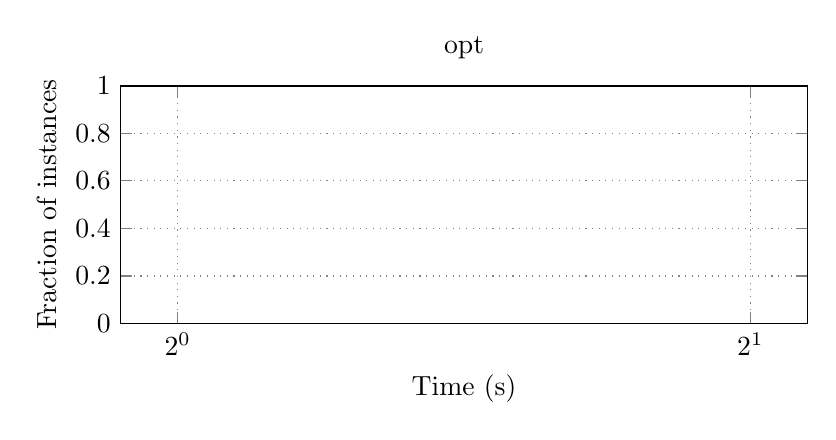
\begin{tikzpicture}
  \begin{axis}[
    my colors,
    title={{opt}},
    xlabel={Time (s)},
    ylabel={Fraction of instances},
    xmode=log,
    log basis x={2},
    ymin=0.1,
    ymax=0.9,
    width=0.85\linewidth,
    height=4.6cm,
    grid=major,
    legend style={
        at={(1.02,0.5)},
        anchor=west,
        font=\small,
    },
    mark=*,
    mark size=0pt,
    line width=0.5pt
    ]
    %% MULTIPLOT({opt})
    %% SELECT x, y, MULTIPLOT FROM (
    %%   SELECT
    %%     total_time AS x,
    %%     (rn) * 1.0 / total_count AS y,
    %%     MULTIPLOT,
    %%     ROW_NUMBER() OVER (PARTITION BY MULTIPLOT, bucket ORDER BY total_time) as row_in_bucket
    %%   FROM (
    %%     SELECT
    %%       total_time,
    %%       RANK() OVER (PARTITION BY MULTIPLOT ORDER BY total_time) as rn,
    %%       COUNT(*) OVER (PARTITION BY MULTIPLOT) as total_count,
    %%       NTILE(500) OVER (PARTITION BY MULTIPLOT ORDER BY total_time) AS bucket,
    %%       MULTIPLOT
    %%     FROM stats
    %%     WHERE init_num_keys >= 1048576 AND index_name = 'DeLI-Static'
    %%   )
    %% )
    %% WHERE row_in_bucket = 1
    %% ORDER BY MULTIPLOT, x
  \end{axis}
\end{tikzpicture}
\end{subfigure}
\newline

%% END FOREACH 
\caption{Performance plots for DeLI-Static index on all workloads and distributions (init key size $2^{i}, i \in [20 , 25]$).}
\end{figure}



\section{DeLI Dynamic}\label{sec:deliconfig}

\subsection{Performance plot (all workloads and distributions)}

\begin{figure}[H]
\small
\centering

%% FOREACH opt IN (RHTOptimization,SIMDLanes,RHTLoad)
\begin{subfigure}{0.4\textwidth}
\centering
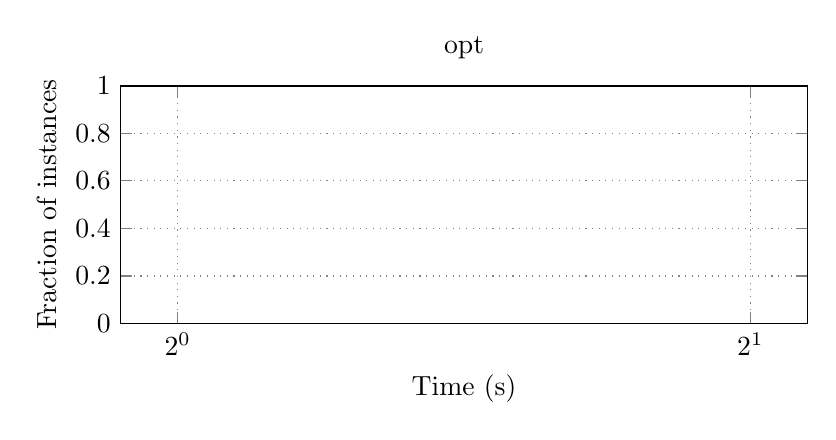
\begin{tikzpicture}
  \begin{axis}[
    my colors,
    title={{opt}},
    xlabel={Time (s)},
    ylabel={Fraction of instances},
    xmode=log,
    log basis x={2},
    ymin=0.1,
    ymax=0.9,
    width=0.85\linewidth,
    height=4.6cm,
    grid=major,
    legend style={
        at={(1.02,0.5)},
        anchor=west,
        font=\small,
    },
    mark=*,
    mark size=0pt,
    line width=0.5pt
    ]
    %% MULTIPLOT({opt})
    %% SELECT x, y, MULTIPLOT FROM (
    %%   SELECT
    %%     total_time AS x,
    %%     (rn) * 1.0 / total_count AS y,
    %%     MULTIPLOT,
    %%     ROW_NUMBER() OVER (PARTITION BY MULTIPLOT, bucket ORDER BY total_time) as row_in_bucket
    %%   FROM (
    %%     SELECT
    %%       total_time,
    %%       RANK() OVER (PARTITION BY MULTIPLOT ORDER BY total_time) as rn,
    %%       COUNT(*) OVER (PARTITION BY MULTIPLOT) as total_count,
    %%       NTILE(500) OVER (PARTITION BY MULTIPLOT ORDER BY total_time) AS bucket,
    %%       MULTIPLOT
    %%     FROM stats
    %%     WHERE init_num_keys >= 1048576 AND index_name = 'DeLI-Dynamic'
    %%   )
    %% )
    %% WHERE row_in_bucket = 1
    %% ORDER BY MULTIPLOT, x
  \end{axis}
\end{tikzpicture}
\end{subfigure}
\newline

%% END FOREACH 
\caption{Performance plots for DeLI-Dynamic index on all workloads and distributions (init key size $2^{i}, i \in [20 , 25]$).}
\end{figure}

\section{DeLI Static Payload}\label{sec:delistaticpayload}

\subsection{Performance plot (all workloads and distributions)}

\begin{figure}[H]
\small
\centering

%% FOREACH opt IN (RHTOptimization,SIMDLanes,RHTLoad,Highbits) SHAREDY
\begin{subfigure}{0.24\textwidth}
\centering
\begin{tikzpicture}
  \begin{axis}[
    title={{opt}},
    xlabel={Time (seconds)},
    ylabel={Fraction of instances},
    xmode=log,
    log basis x={2},
    width=1.2\linewidth,
    height=3.5cm,
    grid=major,
    legend style={
        at={(0.5,-0.2)},
        anchor=north,
    },
    mark=*,
    mark size=0pt,
    line width=0.5pt
    ]
    %% MULTIPLOT({opt})
    %% SELECT x, y, MULTIPLOT FROM (
    %%   SELECT
    %%     total_time AS x,
    %%     (rn) * 1.0 / total_count AS y,
    %%     MULTIPLOT,
    %%     ROW_NUMBER() OVER (PARTITION BY MULTIPLOT, bucket ORDER BY total_time) as row_in_bucket
    %%   FROM (
    %%     SELECT
    %%       total_time,
    %%       RANK() OVER (PARTITION BY MULTIPLOT ORDER BY total_time) as rn,
    %%       COUNT(*) OVER (PARTITION BY MULTIPLOT) as total_count,
    %%       NTILE(500) OVER (PARTITION BY MULTIPLOT ORDER BY total_time) AS bucket,
    %%       MULTIPLOT
    %%     FROM stats
    %%     WHERE init_num_keys >= 1048576 AND index_name = 'DeLI-Static-Payload'
    %%   )
    %% )
    %% WHERE row_in_bucket = 1
    %% ORDER BY MULTIPLOT, x
  \end{axis}
\end{tikzpicture}
\end{subfigure}
\hfill
%% END FOREACH
\caption{Performance plots for DeLI-Static-Payload index on all workloads and distributions (init key size $2^{i}, i \in [20 , 25]$).}
\end{figure}



\section{DeLI Dynamic Payload}\label{sec:delidynamicpayload}

\subsection{Performance plot (all workloads and distributions)}

\begin{figure}[H]
\small
\centering

%% FOREACH opt IN (RHTOptimization,SIMDLanes,RHTLoad,Highbits) SHAREDY
\begin{subfigure}{0.24\textwidth}
\centering
\begin{tikzpicture}
  \begin{axis}[
    title={{opt}},
    xlabel={Time (seconds)},
    ylabel={Fraction of instances},
    xmode=log,
    log basis x={2},
    width=1.2\linewidth,
    height=3.5cm,
    grid=major,
    legend style={
        at={(0.5,-0.2)},
        anchor=north,
    },
    mark=*,
    mark size=0pt,
    line width=0.5pt
    ]
    %% MULTIPLOT({opt})
    %% SELECT x, y, MULTIPLOT FROM (
    %%   SELECT
    %%     total_time AS x,
    %%     (rn) * 1.0 / total_count AS y,
    %%     MULTIPLOT,
    %%     ROW_NUMBER() OVER (PARTITION BY MULTIPLOT, bucket ORDER BY total_time) as row_in_bucket
    %%   FROM (
    %%     SELECT
    %%       total_time,
    %%       RANK() OVER (PARTITION BY MULTIPLOT ORDER BY total_time) as rn,
    %%       COUNT(*) OVER (PARTITION BY MULTIPLOT) as total_count,
    %%       NTILE(500) OVER (PARTITION BY MULTIPLOT ORDER BY total_time) AS bucket,
    %%       MULTIPLOT
    %%     FROM stats
    %%     WHERE init_num_keys >= 1048576 AND index_name = 'DeLI-Dynamic-Payload'
    %%   )
    %% )
    %% WHERE row_in_bucket = 1
    %% ORDER BY MULTIPLOT, x
  \end{axis}
\end{tikzpicture}
\end{subfigure}
\hfill
%% END FOREACH
\caption{Performance plots for DeLI-Dynamic-Payload index on all workloads and distributions (init key size $2^{i}, i \in [20 , 25]$).}
\end{figure}

\section{Best Variants Performance}\label{sec:best}

\subsection{Performance plot (best variant per index)}

\begin{figure}[H]
\small
\centering
\begin{tikzpicture}
  \begin{axis}[
    title={Best variants},
    xlabel={Time (seconds)},
    ylabel={Fraction of instances},
    xmode=log,
    log basis x={2},
    width=150mm,
    height=100mm,
    grid=major,
    legend pos=south east,
    mark=*,
    mark size=0pt,
    line width=0.5pt
    ]
    %% MULTIPLOT(index_name)
    %% SELECT x, y, MULTIPLOT FROM (
    %%   SELECT
    %%     total_time AS x,
    %%     (rn) * 1.0 / total_count AS y,
    %%     MULTIPLOT,
    %%     ROW_NUMBER() OVER (PARTITION BY MULTIPLOT, bucket ORDER BY total_time) as row_in_bucket
    %%   FROM (
    %%     SELECT
    %%       total_time,
    %%       RANK() OVER (PARTITION BY MULTIPLOT ORDER BY total_time) as rn,
    %%       COUNT(*) OVER (PARTITION BY MULTIPLOT) as total_count,
    %%       NTILE(1000) OVER (PARTITION BY MULTIPLOT ORDER BY total_time) AS bucket,
    %%       MULTIPLOT
    %%     FROM stats_best
    %%     WHERE init_num_keys >= 1048576
    %%   )
    %% )
    %% WHERE row_in_bucket = 1
    %% ORDER BY MULTIPLOT, x
  \end{axis}
\end{tikzpicture}
\caption{Performance plots for best index variants (init key size $2^{i}, i \in [20 , 25]$).}
\end{figure}

\end{document}
